% Gabarit pandoc des corrigés publiés (brut et guidé). Contenu sans marque ni nom de site.
% Compilation : lualatex (latexmk -lualatex).
% Le Markdown reste la source unique : ne pas éditer ce fichier .tex à la main.
\documentclass[11pt,a4paper]{article}

% --- Moteur, polices (Latin Modern) et langue ---------------------------------
\usepackage{iftex}
\ifLuaTeX\else\errmessage{Ce document se compile avec lualatex}\fi
\usepackage{amsmath,amssymb,mathtools}
\usepackage{fontspec}
% mathrm=sym : \mathrm prend ses glyphes dans la police mathématique (ℓ, μ, Ω), comme KaTeX.
\usepackage[math-style=TeX,bold-style=TeX,mathrm=sym]{unicode-math}
% Repli pour les glyphes absents de Latin Modern (indices et exposants Unicode,
% flèches, filets des schémas en texte, symboles) : DejaVu, puis Latin Modern Math
% (ℓ, lettres mathématiques Unicode des légendes).
\directlua{
  luaotfload.add_fallback("repliTexte", {"DejaVuSerif:mode=harf;", "DejaVuSans:mode=harf;", "file:latinmodern-math.otf:mode=harf;"})
  luaotfload.add_fallback("repliMono", {"DejaVuSansMono:mode=harf;", "DejaVuSans:mode=harf;", "file:latinmodern-math.otf:mode=harf;"})
}
\setmainfont{Latin Modern Roman}[RawFeature={fallback=repliTexte}]
\setsansfont{Latin Modern Sans}[RawFeature={fallback=repliTexte}]
\setmonofont{Latin Modern Mono}[RawFeature={fallback=repliMono}]
\setmathfont{Latin Modern Math}
\usepackage[french]{babel}
\frenchsetup{SmallCapsFigTabCaptions=false}

% --- Mise en page --------------------------------------------------------------
\usepackage[a4paper,margin=2.2cm,headheight=14pt,footskip=1.2cm]{geometry}
\usepackage{microtype}
\setlength{\emergencystretch}{4em}
\tolerance=1500
\setlength{\parindent}{0pt}
\setlength{\parskip}{0.55\baselineskip plus 2pt minus 1pt}
\usepackage{xcolor}
% Gris nommés : babel-french rend « ! » actif dans le document.
\definecolor{gris2}{gray}{0.98}
\definecolor{gris3}{gray}{0.97}
\definecolor{gris5}{gray}{0.95}
\definecolor{gris35}{gray}{0.65}
\definecolor{gris40}{gray}{0.60}
\definecolor{gris45}{gray}{0.55}
\definecolor{gris50}{gray}{0.50}
\definecolor{gris55}{gray}{0.45}
\definecolor{gris60}{gray}{0.40}
\definecolor{gris65}{gray}{0.35}
\definecolor{gris70}{gray}{0.30}
\definecolor{gris80}{gray}{0.20}
\definecolor{gris85}{gray}{0.15}
\usepackage{graphicx}
\usepackage{float}
\usepackage{caption}
\captionsetup{font=small,labelformat=empty,justification=centering}
\usepackage{booktabs,longtable,array,multirow,calc}
\usepackage{siunitx}
\sisetup{locale=FR}
\usepackage[version=4]{mhchem}
\usepackage{listings}
\usepackage{fancyhdr}
\usepackage{lastpage}
\usepackage[most]{tcolorbox}
\usepackage{enumitem}
\setlist{nosep,leftmargin=*,topsep=2pt}
\usepackage[hidelinks,unicode]{hyperref}
\usepackage{bookmark}
\hypersetup{pdftitle={Centrale-Supélec TSI — Mathématiques 2 2026},pdfauthor={Rédigé par IA},pdfcreator={LaTeX},pdfsubject={Corrigé brut}}
\usepackage{xurl}

% --- Pandoc : listes, tableaux, figures ----------------------------------------
\providecommand{\passthrough}[1]{#1}
\providecommand{\tightlist}{\setlength{\itemsep}{0pt}\setlength{\parskip}{0pt}}

\makeatletter
\def\maxwidth{\ifdim\Gin@nat@width>\linewidth\linewidth\else\Gin@nat@width\fi}
\def\maxheight{\ifdim\Gin@nat@height>0.55\textheight 0.55\textheight\else\Gin@nat@height\fi}
\makeatother
\setkeys{Gin}{width=\maxwidth,height=\maxheight,keepaspectratio}
\setcounter{secnumdepth}{-\maxdimen}
\providecommand{\pandocbounded}[1]{#1}
\usepackage{longtable,booktabs,array}

% --- Code (listings) -----------------------------------------------------------
\lstset{
  basicstyle=\ttfamily\small,
  columns=fullflexible,
  keepspaces=true,
  breaklines=true,
  breakatwhitespace=false,
  postbreak=\mbox{\textcolor{gris50}{$\hookrightarrow$}\space},
  frame=single,
  rulecolor=\color{gris35},
  framesep=4pt,
  xleftmargin=5pt,xrightmargin=5pt,
  backgroundcolor=\color{gris3},
  keywordstyle=\bfseries,
  commentstyle=\color{gris65},
  stringstyle=\color{gris80},
  showstringspaces=false,
  tabsize=4,
  extendedchars=true,
  aboveskip=6pt,belowskip=6pt,
}

% --- Macros des corrigés (KaTeX ↔ LaTeX) ---------------------------------------
% Les corrigés sont écrits pour KaTeX : on définit ici ce que KaTeX connaît et
% que LaTeX n'a pas, sans jamais retoucher le Markdown.
\providecommand{\R}{\mathbb{R}}
\providecommand{\N}{\mathbb{N}}
\providecommand{\Z}{\mathbb{Z}}
\providecommand{\Q}{\mathbb{Q}}
\providecommand{\C}{\mathbb{C}}
\providecommand{\dd}{\mathrm{d}}
\providecommand{\llbracket}{\lBrack}
\providecommand{\rrbracket}{\rBrack}
\providecommand{\lBrace}{\lbrace}
\providecommand{\rBrace}{\rbrace}
\providecommand{\Box}{\square}
\providecommand{\Diamond}{\lozenge}
\providecommand{\varnothing}{\emptyset}
\providecommand{\argmax}{\operatorname*{arg\,max}}
\providecommand{\argmin}{\operatorname*{arg\,min}}
\renewcommand{\leq}{\leqslant}
\renewcommand{\geq}{\geqslant}

% Équation hors texte : réduite à la largeur de la ligne si elle déborde.
\newsavebox{\boiteequation}
\newcommand{\equationajustee}[1]{%
  \sbox{\boiteequation}{$\displaystyle #1$}%
  \ifdim\wd\boiteequation>\linewidth
    \[\resizebox{\linewidth}{!}{\usebox{\boiteequation}}\]%
  \else
    \[#1\]%
  \fi}

% --- Encadrés pédagogiques (sobres, lisibles en noir et blanc) -----------------
\tcbset{
  encadre/.style={
    enhanced,breakable,sharp corners,
    colback=white,colframe=gris55,
    boxrule=0.4pt,leftrule=2.2pt,
    left=6pt,right=6pt,top=3pt,bottom=3pt,
    before skip=6pt,after skip=6pt,
    fonttitle=\bfseries\small,coltitle=black,
    attach title to upper,after title={\quad},
    parbox=false,
  }
}
\newtcolorbox{indication}[1]{encadre,colframe=gris45,colback=gris2,title={Indication~#1}}
\newtcolorbox{methode}{encadre,colframe=gris70,title={Méthode}}
\newtcolorbox{piege}{encadre,colframe=gris85,boxrule=0.8pt,leftrule=2.2pt,title={Piège}}
\newtcolorbox{jury}{encadre,colframe=gris60,colback=gris5,title={Jury}}
\newtcolorbox{encadrenote}{encadre,colframe=gris40}

% --- Titres de section ---------------------------------------------------------
\usepackage{titlesec}
\titleformat{\section}{\Large\bfseries}{}{0pt}{}
\titleformat{\subsection}{\large\bfseries}{}{0pt}{}
\titleformat{\subsubsection}{\normalsize\bfseries}{}{0pt}{}
\titlespacing*{\section}{0pt}{14pt plus 4pt minus 2pt}{6pt}
\titlespacing*{\subsection}{0pt}{10pt plus 3pt minus 2pt}{4pt}
\titlespacing*{\subsubsection}{0pt}{8pt plus 2pt minus 2pt}{2pt}

% --- En-tête et pied de page ---------------------------------------------------
\pagestyle{fancy}
\fancyhf{}
\fancyhead[L]{\small\textsc{Corrigé brut} · Centrale-Supélec TSI}
\fancyhead[R]{\small Maths 2 2026}
\fancyfoot[L]{\footnotesize Corrigé rédigé par IA, non officiel}
\fancyfoot[R]{\footnotesize \thepage\,/\,\pageref*{LastPage}}
\renewcommand{\headrulewidth}{0.4pt}
\renewcommand{\footrulewidth}{0pt}
\fancypagestyle{plain}{\fancyhf{}\fancyfoot[R]{\footnotesize \thepage\,/\,\pageref*{LastPage}}\fancyfoot[L]{\footnotesize Corrigé rédigé par IA, non officiel}\renewcommand{\headrulewidth}{0pt}}

\begin{document}
\thispagestyle{plain}
\begin{center}
  {\small\scshape Corrigé brut}\par\smallskip
  {\LARGE\bfseries Centrale-Supélec TSI — Mathématiques 2 2026\par}\medskip
  {\large Centrale-Supélec · TSI · Maths 2 · 2026\par}
\end{center}
\vspace{2pt}\hrule\vspace{8pt}

\emph{Corrigé rédigé par IA, non officiel. Signalez toute erreur.}

Notations : \(\binom{j}{i}=0\) si \(i>j\) (convention de l'énoncé). Deux défauts de l'énoncé sont corrigés en place. En \textbf{Q31}, « la matrice introduite en Q25 » désigne la matrice de la figure 4, introduite en \textbf{Q26}. En \textbf{Q37}, la convention cohérente est \textbf{\(b_0=1\)} et non \(b_0=0\).

\hypertarget{partie-a-matrices-de-pascal}{%
\section{Partie A --- Matrices de Pascal}\label{partie-a-matrices-de-pascal}}

\hypertarget{i-cas-particulier-n2}{%
\subsection{\texorpdfstring{I --- Cas particulier \(n=2\)}{I --- Cas particulier n=2}}\label{i-cas-particulier-n2}}

\hypertarget{question-1}{%
\subsection{Question 1}\label{question-1}}

Pour \(P=a+bX+cX^2\in\mathbb R_2[X]\) :
\equationajustee{\begin{aligned}
u(P)&=a+b(X+1)+c(X+1)^2\\
&=(a+b+c)+(b+2c)X+cX^2\in\mathbb R_2[X].
\end{aligned}}
Soient \(P,Q\in\mathbb R_2[X]\) et \(\lambda,\mu\in\mathbb R\). Alors \((\lambda P+\mu Q)(X+1)=\lambda P(X+1)+\mu Q(X+1)\), donc \(u\) est linéaire. C'est un endomorphisme de \(\mathbb R_2[X]\).

\(u(1)=1\), \(u(X)=1+X\), \(u(X^2)=1+2X+X^2\). En rangeant ces coordonnées en colonnes :
\equationajustee{\boxed{\operatorname{Mat}_e(u)=\begin{pmatrix}1&1&1\\0&1&2\\0&0&1\end{pmatrix}.}}

\hypertarget{question-2}{%
\subsection{Question 2}\label{question-2}}

Notons \(A=\operatorname{Mat}_e(u)\). Elle est triangulaire, donc \(\det A=1\neq0\) : \(A\) est inversible.

Soit \(v:P\mapsto P(X-1)\) sur \(\mathbb R_2[X]\). Pour tout \(P\) :
\equationajustee{\begin{aligned}
u(v(P))&=P((X+1)-1)\\
&=P,\\[4pt]
v(u(P))&=P.
\end{aligned}}
Donc \(v=u^{-1}\) et \(A^{-1}=\operatorname{Mat}_e(v)\). Comme \(v(1)=1\), \(v(X)=-1+X\) et \(v(X^2)=1-2X+X^2\) :
\equationajustee{\boxed{A^{-1}=\begin{pmatrix}1&-1&1\\0&1&-2\\0&0&1\end{pmatrix}.}}

\(A\) est triangulaire : ses valeurs propres sont ses coefficients diagonaux, \(\boxed{\operatorname{Sp}(A)=\{1\}}\).

Si \(A\) était diagonalisable, elle serait semblable à \(\operatorname{diag}(1,1,1)=I_3\), donc \(A=PI_3P^{-1}=I_3\). C'est faux, car \(A_{1,2}=1\). \textbf{\(A\) n'est pas diagonalisable.}

De façon équivalente : \(\operatorname{rg}(A-I_3)=2\), donc \(\dim\ker(A-I_3)=1<3\).

\hypertarget{ii-des-matrices-semblables-uxe0-leurs-inverses}{%
\subsection{II --- Des matrices semblables à leurs inverses}\label{ii-des-matrices-semblables-uxe0-leurs-inverses}}

\hypertarget{question-3}{%
\subsection{Question 3}\label{question-3}}

Pour \(j\in[\![0,n]\!]\), la formule du binôme donne
\equationajustee{\begin{aligned}
u(X^j)&=(X+1)^j\\
&=\sum_{i=0}^{j}\binom{j}{i}X^i.
\end{aligned}}
La colonne \(j\) de \(U\) a donc pour coefficients \(\binom{j}{i}\), nuls pour \(i>j\) :
\equationajustee{\boxed{\forall (i,j)\in[\![0,n]\!]^2,\quad U_{i,j}=\binom{j}{i},}}
et \textbf{\(U\) est triangulaire supérieure}, de coefficients diagonaux \(\binom ii=1\). Donc \(\operatorname{Sp}(U)=\{1\}\).

\begin{itemize}
\tightlist
\item
  Si \(n=0\), \(U=(1)\) est diagonale.
\item
  Si \(n\ge1\) : \(U\) diagonalisable de spectre \(\{1\}\) serait semblable, donc égale, à \(I_{n+1}\). Or \(U_{0,1}=\binom10=1\). \textbf{Dans ce cas, \(U\) n'est pas diagonalisable.}
\end{itemize}

\hypertarget{question-4}{%
\subsection{Question 4}\label{question-4}}

Pour tout \(P\in\mathbb R_n[X]\), \((u\circ v)(P)=P((X-1)+1)=P\). Donc
\equationajustee{\boxed{u\circ v={\mathrm{id}}_{\mathbb R_n[X]}},}
et de même \(v\circ u=\mathrm{id}\).

Ainsi \(u\) est bijective, d'inverse \(v\). Par suite \(U\) est inversible et \(U^{-1}=\operatorname{Mat}_e(v)\). Comme
\equationajustee{\begin{aligned}
v(X^j)&=(X-1)^j\\
&=\sum_{i=0}^{j}\binom{j}{i}(-1)^{j-i}X^i,
\end{aligned}}
on obtient
\equationajustee{\boxed{\forall (i,j)\in[\![0,n]\!]^2,\quad (U^{-1})_{i,j}=(-1)^{j-i}\binom{j}{i}.}}
Pour \(n=2\), cette formule donne
\equationajustee{U^{-1}=\begin{pmatrix}1&-1&1\\0&1&-2\\0&0&1\end{pmatrix}.}
C'est la matrice obtenue en Q2 : \textbf{le résultat est cohérent}.

\hypertarget{question-5}{%
\subsection{Question 5}\label{question-5}}

\(D\) est diagonale de coefficients \((-1)^i\). Donc \(D^2\) est diagonale de coefficients \(((-1)^i)^2=1\), c'est-à-dire
\equationajustee{D^2=I_{n+1}.}
Ainsi \(D\) est inversible et \(\boxed{D^{-1}=D}\).

\hypertarget{question-6}{%
\subsection{Question 6}\label{question-6}}

Multiplier à gauche par \(D\) multiplie la ligne \(i\) par \((-1)^i\) ; multiplier à droite multiplie la colonne \(j\) par \((-1)^j\). Pour \((i,j)\in[\![0,n]\!]^2\) :
\equationajustee{\begin{aligned}
(DU)_{i,j}&=(-1)^i\binom ji,\\[4pt]
(U^{-1}D)_{i,j}&=(-1)^{j-i}\binom ji(-1)^j\\
&=(-1)^{2j-i}\binom ji\\
&=(-1)^i\binom ji.
\end{aligned}}
Donc \(\boxed{DU=U^{-1}D}\). En multipliant à gauche par \(D\) et en utilisant \(D^2=I_{n+1}\), on obtient \(U=DU^{-1}D\). Comme \(D=D^{-1}\) :
\equationajustee{\boxed{U=DU^{-1}D^{-1}.}}
\(D\) étant inversible, \textbf{\(U\) est semblable à \(U^{-1}\)}.

\hypertarget{question-7}{%
\subsection{Question 7}\label{question-7}}

On a \(D^\top=D\). Comme \(U\) est inversible, \(L=U^\top\) l'est aussi et \((U^{-1})^\top=(U^\top)^{-1}=L^{-1}\). En transposant \(U=DU^{-1}D\) :
\equationajustee{\begin{aligned}
L&=U^\top\\
&=D^\top(U^{-1})^\top D^\top\\
&=DL^{-1}D.
\end{aligned}}
Comme \(D=D^{-1}\) :
\equationajustee{\boxed{L=DL^{-1}D=DL^{-1}D^{-1}},}
donc \textbf{\(L\) est semblable à \(L^{-1}\)}.

On note pour la suite : \(L_{i,j}=\binom ij\) et \((L^{-1})_{i,j}=(-1)^{i-j}\binom ij\).

\hypertarget{iii-une-matrice-diagonalisable-semblable-uxe0-son-inverse}{%
\subsection{III --- Une matrice diagonalisable semblable à son inverse}\label{iii-une-matrice-diagonalisable-semblable-uxe0-son-inverse}}

\hypertarget{question-8}{%
\subsection{Question 8}\label{question-8}}

Pour \(n=2\), \(L=\begin{pmatrix}1&0&0\\1&1&0\\1&2&1\end{pmatrix}\) et
\equationajustee{\boxed{S=LU=\begin{pmatrix}1&1&1\\1&2&3\\1&3&6\end{pmatrix}.}}
\(S^\top=U^\top L^\top=LU=S\) : \(S\) est symétrique réelle, donc \textbf{diagonalisable} par le théorème spectral.

En développant selon la première ligne :
\equationajustee{\begin{aligned}
\chi_S(X)&=\det\begin{pmatrix}X-1&-1&-1\\-1&X-2&-3\\-1&-3&X-6\end{pmatrix}\\
&=(X-1)(X^2-8X+3)-(X-3)-(X+1)\\
&=(X-1)(X^2-8X+1).
\end{aligned}}
Contrôles : le coefficient de \(X^2\) vaut \(-9=-\operatorname{tr}S\). De plus \(\chi_S(0)=-1=-\det S\), car \(\det S=\det L\det U=1\).

Le trinôme \(X^2-8X+1\) a pour discriminant \(60\). Ses racines sont \(4\pm\sqrt{15}\), de produit \(1\). Avec \(\alpha=4+\sqrt{15}>1\), l'autre racine est \(\frac1\alpha=4-\sqrt{15}\) :
\equationajustee{\boxed{\operatorname{Sp}(S)=\left\{1,\ \alpha,\ \tfrac1\alpha\right\}}}
avec \(\alpha=4+\sqrt{15}>1\).

\hypertarget{question-9}{%
\subsection{Question 9}\label{question-9}}

\begin{itemize}
\tightlist
\item
  \(S^\top=(LU)^\top=U^\top L^\top=LU=S\) : \(S\) est symétrique réelle, donc \textbf{diagonalisable} (théorème spectral).
\item
  \(S=LU\) est un produit de matrices inversibles : \textbf{\(S\) est inversible} et \(S^{-1}=U^{-1}L^{-1}\).
\item
  De Q7, \(LD=DL^{-1}D^2=DL^{-1}\). Avec \(DU=U^{-1}D\) (Q6) et \(D^{-1}=D\) :
  \equationajustee{\begin{aligned}
  (DU)S(DU)^{-1}&=DU\,LU\,U^{-1}D\\
  &=(DU)(LD)\\
  &=(U^{-1}D)(DL^{-1})\\
  &=U^{-1}L^{-1}\\
  &=S^{-1}.
  \end{aligned}}
\end{itemize}

Donc \(\boxed{S^{-1}=(DU)S(DU)^{-1}}\) avec \(DU\) inversible : \textbf{\(S\) est semblable à son inverse}.

\hypertarget{question-10}{%
\subsection{Question 10}\label{question-10}}

Soit \(\lambda\) une valeur propre de \(S\) (réelle, \(S\) étant symétrique réelle) et \(X\neq0\) tel que \(SX=\lambda X\).

\begin{itemize}
\tightlist
\item
  D'une part, \(X^\top SX=\lambda X^\top X=\lambda\|X\|^2\) avec \(\|X\|^2=\sum_i x_i^2>0\).
\item
  D'autre part, \(S=U^\top U\), donc \(X^\top SX=(UX)^\top(UX)=\|UX\|^2\). Et \(UX\neq0\), car \(U\) est inversible et \(X\neq0\).
\end{itemize}

Donc \(\lambda=\dfrac{\|UX\|^2}{\|X\|^2}\) et \(\boxed{\lambda>0}\).

\hypertarget{question-11}{%
\subsection{Question 11}\label{question-11}}

D'après Q10, \(0\notin\operatorname{Sp}(S)\) : la fonction \(x\mapsto\frac1x\) est définie sur \(\operatorname{Sp}(S)\).

Soit \(\lambda\in\operatorname{Sp}(S)\) et \(X\neq0\) tel que \(SX=\lambda X\). Alors \(S^{-1}X=\frac1\lambda X\), donc \(\frac1\lambda\in\operatorname{Sp}(S^{-1})\).

Or \(S^{-1}\) et \(S\) sont semblables (Q9) : elles ont le même polynôme caractéristique, donc le même spectre. Ainsi \(\frac1\lambda\in\operatorname{Sp}(S)\).

\textbf{\(\operatorname{Sp}(S)\) est stable par \(x\mapsto\frac1x\).}

\hypertarget{question-12}{%
\subsection{Question 12}\label{question-12}}

\(A\) est inversible, d'inverse \(A^{-1}=\operatorname{diag}(\frac12,\frac12,2)\). Son spectre \(\operatorname{Sp}(A)=\{2,\frac12\}\) est stable par \(x\mapsto\frac1x\). Mais
\equationajustee{\begin{aligned}
\operatorname{tr}A&=\tfrac92,\\
\operatorname{tr}A^{-1}&=3,
\end{aligned}}
et deux matrices semblables ont la même trace (\(\operatorname{tr}(PAP^{-1})=\operatorname{tr}(P^{-1}PA)=\operatorname{tr}A\)). Donc \(A\) n'est pas semblable à \(A^{-1}\).

\textbf{Non} : une matrice inversible dont le spectre est stable par \(x\mapsto\frac1x\) n'est pas toujours semblable à son inverse.

\hypertarget{iv-calcul-des-coefficients-de-s-uxe0-laide-dun-duxe9nombrement-dans-un-graphe}{%
\subsection{\texorpdfstring{IV --- Calcul des coefficients de \(S\) à l'aide d'un dénombrement dans un graphe}{IV --- Calcul des coefficients de S à l'aide d'un dénombrement dans un graphe}}\label{iv-calcul-des-coefficients-de-s-uxe0-laide-dun-duxe9nombrement-dans-un-graphe}}

\hypertarget{question-13}{%
\subsection{Question 13}\label{question-13}}

On suppose \(n\ge2\). Après l'arc \(s\to(0,0)\), un chemin vers \((2,2)\) comporte deux arcs « bas » \((i,j)\to(i+1,j)\) et deux arcs « droite » \((i,j)\to(i,j+1)\), dans un ordre quelconque :
\equationajustee{\Omega_{2,2}=\left\{\begin{aligned}{}&s\to(0,0)\to(1,0)\to(2,0)\to(2,1)\to(2,2),\\
&s\to(0,0)\to(1,0)\to(1,1)\to(2,1)\to(2,2),\\
&s\to(0,0)\to(1,0)\to(1,1)\to(1,2)\to(2,2),\\
&s\to(0,0)\to(0,1)\to(1,1)\to(2,1)\to(2,2),\\
&s\to(0,0)\to(0,1)\to(1,1)\to(1,2)\to(2,2),\\
&s\to(0,0)\to(0,1)\to(0,2)\to(1,2)\to(2,2)
\end{aligned}\right\}.}
Donc \(|\Omega_{2,2}|=6=\binom42\).

Cas général. Chaque arc autre que \(s\to(0,0)\) augmente de \(1\) exactement une coordonnée.

Un chemin de \(s\) à \((i,j)\) commence donc par \(s\to(0,0)\). Il se poursuit par \(i+j\) arcs, dont \(i\) « bas » et \(j\) « droite ».

À un chemin, on associe l'ensemble des rangs (dans \([\![1,i+j]\!]\)) de ses arcs « bas ». Cette application est :

\begin{itemize}
\tightlist
\item
  injective, car cet ensemble fixe la suite des déplacements, donc celle des sommets ;
\item
  surjective : soit une partie à \(i\) éléments de \([\![1,i+j]\!]\). Elle définit une suite de déplacements de \((0,0)\) à \((i,j)\). Les sommets visités ont leurs coordonnées dans \([\![0,\max(i,j)]\!]\subset[\![0,n]\!]\) : c'est un chemin de \(G_n\).
\end{itemize}

C'est une bijection vers les parties à \(i\) éléments d'un ensemble à \(i+j\) éléments :
\equationajustee{\boxed{\forall(i,j)\in[\![0,n]\!]^2,\quad |\Omega_{i,j}|=\binom{i+j}{i}.}}

\hypertarget{question-14}{%
\subsection{Question 14}\label{question-14}}

On munit \(\Omega_{i,j}\) de la probabilité uniforme. Soit \(k\in[\![0,i]\!]\) ; le sommet \((k,i-k)\) est dans \([\![0,n]\!]^2\).

Un chemin de \(A_k\) se coupe de façon unique en deux morceaux. Le premier va de \(s\) au sommet \((k,i-k)\). Le second va de ce sommet à \((i,j)\). Réciproquement, toute telle concaténation est dans \(A_k\).

\begin{itemize}
\item
  Chemins de \(s\) à \((k,i-k)\) : \(\binom{k+(i-k)}{k}=\binom ik\) (Q13).
\item
  Chemins de \((k,i-k)\) à \((i,j)\). Chacun comporte \(i-k\) arcs « bas » et \(j-(i-k)\) arcs « droite », soit \(j\) arcs. Le même argument qu'en Q13 en donne \(\binom{j}{i-k}\).

  Si \(i-k>j\), il n'y en a aucun, car la seconde coordonnée ne décroît pas. C'est conforme à \(\binom j{i-k}=0\).
\end{itemize}

\equationajustee{\boxed{|A_k|=\binom ik\binom j{i-k}.}}

Système complet. Le long d'un chemin de \(\Omega_{i,j}\), la somme des coordonnées vaut \(0\) en \((0,0)\). Elle augmente de \(1\) à chaque arc, jusqu'à \(i+j\ge i\).

Le chemin passe donc par un et un seul sommet de somme \(i\). Ce sommet s'écrit \((k,i-k)\) avec \(0\le k\le i\) (la première coordonnée croît jusqu'à \(i\)).

Chaque chemin appartient ainsi à exactement un \(A_k\). Les \(A_k\), pour \(k\in[\![0,i]\!]\), sont deux à deux incompatibles et de réunion \(\Omega_{i,j}\) : \textbf{ils forment un système complet d'événements}. Par conséquent :
\equationajustee{\begin{aligned}
\binom{i+j}{i}&=|\Omega_{i,j}|\\
&=\sum_{k=0}^{i}|A_k|,
\end{aligned}}
c'est-à-dire
\equationajustee{\boxed{\binom{i+j}{i}=\sum_{k=0}^{i}\binom ik\binom j{i-k}.}}

\begin{figure}[H]
\centering
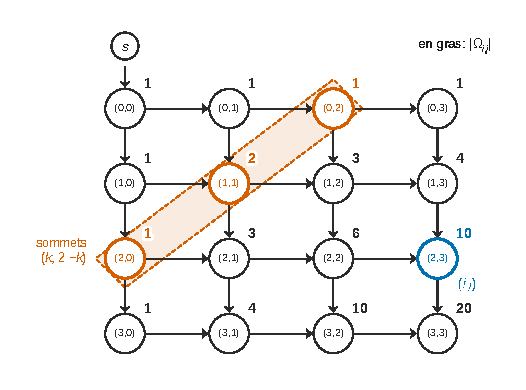
\includegraphics{figures/q14-graphe-chemins.pdf}
\caption*{Figure 1 --- Graphe G₃ annoté : à chaque sommet (i, j), le nombre de
chemins C(i+j, i) ; tout chemin vers (2, 3) traverse un seul sommet (k,
2 − k)}
\end{figure}

\hypertarget{question-15}{%
\subsection{Question 15}\label{question-15}}

Comme \(L_{i,k}=U_{k,i}=\binom ik\) et \(U_{k,j}=\binom jk\) :
\equationajustee{\begin{aligned}
S_{i,j}&=\sum_{k=0}^{n}\binom ik\binom jk\\
&=\sum_{k=0}^{i}\binom i{i-k}\binom jk\\
&=\sum_{m=0}^{i}\binom im\binom j{i-m}
\end{aligned}}
(termes nuls pour \(k>i\), symétrie \(\binom ik=\binom i{i-k}\) pour \(0\le k\le i\), puis \(m=i-k\)). D'après Q14 :
\equationajustee{\boxed{\forall (i,j)\in[\![0,n]\!]^2,\quad S_{i,j}=\binom{i+j}{i}.}}
Pour \(n=2\) on retrouve la matrice de Q8.

\hypertarget{partie-b-uxe9tude-dune-suite-et-dune-suxe9rie-entiuxe8re}{%
\section{Partie B --- Étude d'une suite et d'une série entière}\label{partie-b-uxe9tude-dune-suite-et-dune-suxe9rie-entiuxe8re}}

\hypertarget{i-uxe9tude-dune-suite}{%
\subsection{I --- Étude d'une suite}\label{i-uxe9tude-dune-suite}}

\hypertarget{question-16}{%
\subsection{Question 16}\label{question-16}}

\(a_2=1\cdot(a_1+a_0)=1\) et \(a_3=2(a_2+a_1)=2\) : \(\boxed{a_2=1,\ a_3=2.}\)

\hypertarget{question-17}{%
\subsection{Question 17}\label{question-17}}

\begin{lstlisting}[language=Python]
def liste_an(n):
    """Renvoie la liste [a_0, a_1, ..., a_n]."""
    if n == 0:
        return [1]
    a = [1, 0]
    for k in range(1, n):          # ajoute a_{k+1} = k * (a_k + a_{k-1})
        a.append(k * (a[k] + a[k - 1]))
    return a
\end{lstlisting}

Avant l'itération d'indice \(k\), \texttt{a} vaut \([a_0,\dots,a_k]\). Après la dernière (\(k=n-1\)), elle vaut \([a_0,\dots,a_n]\). \texttt{liste\_an(6)} renvoie \texttt{{[}1,\allowbreak{}\ 0,\allowbreak{}\ 1,\allowbreak{}\ 2,\allowbreak{}\ 9,\allowbreak{}\ 44,\allowbreak{}\ 265{]}\allowbreak{}}.

\hypertarget{question-18}{%
\subsection{Question 18}\label{question-18}}

Soit \(\mathcal P(n)\) : « \(a_n\in\mathbb N\) et \(a_{n+1}\in\mathbb N\) ».

\begin{itemize}
\tightlist
\item
  \(\mathcal P(0)\) est vraie, car \(a_0=1\) et \(a_1=0\).
\item
  Si \(\mathcal P(n)\) est vraie, \(a_{n+2}=(n+1)(a_{n+1}+a_n)\) est un entier naturel, comme produit et somme d'entiers naturels. Donc \(\mathcal P(n+1)\) est vraie.
\end{itemize}

Par récurrence, \(\boxed{\forall n\in\mathbb N,\ a_n\in\mathbb N.}\)

\hypertarget{question-19}{%
\subsection{Question 19}\label{question-19}}

Soit \(\mathcal Q(n)\) : « \(a_n\le n!\) et \(a_{n+1}\le(n+1)!\) ».

\(\mathcal Q(0)\) est vraie (\(1\le1\), \(0\le1\)). Si \(\mathcal Q(n)\) est vraie, comme \(n+1>0\) :
\equationajustee{\begin{aligned}
a_{n+2}&=(n+1)(a_{n+1}+a_n)\\
&\le(n+1)\big((n+1)!+n!\big)\\
&=(n+1)\,n!\,(n+2)\\
&=(n+2)!.
\end{aligned}}
Par récurrence, \(\boxed{\forall n\in\mathbb N,\ a_n\le n!.}\)

\hypertarget{question-20}{%
\subsection{Question 20}\label{question-20}}

Le développement \(e^x=\sum_{k=0}^{+\infty}\frac{x^k}{k!}\) est valable pour tout réel \(x\). En \(x=-1\), il montre que la série \(\sum\frac{(-1)^k}{k!}\) \textbf{converge}, et
\equationajustee{\boxed{\sum_{k=0}^{+\infty}\frac{(-1)^k}{k!}=\frac1e,}}
c'est-à-dire \(S_n\xrightarrow[n\to+\infty]{}\frac1e\).

Pour \(p\in\mathbb N\) :
\equationajustee{\begin{aligned}
S_{2p+2}-S_{2p}&=\frac1{(2p+2)!}-\frac1{(2p+1)!}\\
&\le0,\\[4pt]
S_{2p+3}-S_{2p+1}&=\frac1{(2p+2)!}-\frac1{(2p+3)!}\\
&\ge0,\\[4pt]
S_{2p}-S_{2p+1}&=\frac1{(2p+1)!}\\
&\xrightarrow[p\to+\infty]{}0.
\end{aligned}}
Les suites \((S_{2p})\) (décroissante) et \((S_{2p+1})\) (croissante) sont donc adjacentes. Leur limite commune est \(\frac1e\), et \(S_{2p+1}\le\frac1e\le S_{2p}\) pour tout \(p\). Ainsi, pour tout \(n\in\mathbb N\) :
\equationajustee{\boxed{\begin{aligned}{}&S_n\le\frac1e\le S_{n+1}&&\text{si }n\text{ est impair,}\\
&S_{n+1}\le\frac1e\le S_n&&\text{si }n\text{ est pair.}
\end{aligned}}}
Dans les deux cas, \(\frac1e\) est compris entre \(S_n\) et \(S_{n+1}\). D'où
\equationajustee{\begin{aligned}
\left|\frac1e-S_n\right|&\le|S_{n+1}-S_n|\\
&=\frac1{(n+1)!}.
\end{aligned}}

\begin{figure}[H]
\centering
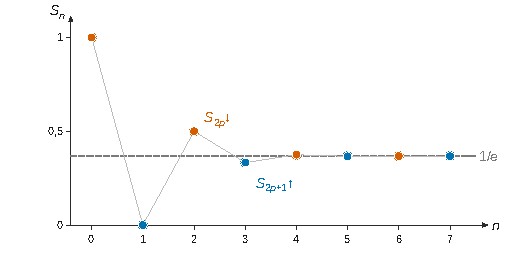
\includegraphics{figures/q20-sommes-partielles.pdf}
\caption*{Figure 2 --- Sommes partielles S\_n : les rangs pairs décroissent
au-dessus de 1/e, les rangs impairs croissent au-dessous}
\end{figure}

\hypertarget{question-21}{%
\subsection{Question 21}\label{question-21}}

Soit \(\mathcal R(n)\) : « \(a_n=n!S_n\) et \(a_{n+1}=(n+1)!S_{n+1}\) ».

Initialisation : \(0!S_0=1=a_0\) et \(1!S_1=0=a_1\).

Hérédité : supposons \(\mathcal R(n)\) vraie. Comme \(n!S_n=n!S_{n+1}-\frac{(-1)^{n+1}}{n+1}\), on obtient :
\equationajustee{\begin{aligned}
a_{n+2}&=(n+1)\left((n+1)!S_{n+1}+n!S_{n+1}-\frac{(-1)^{n+1}}{n+1}\right)\\
&=(n+1)\,n!\,(n+2)\,S_{n+1}+(-1)^{n+2}\\
&=(n+2)!\left(S_{n+1}+\frac{(-1)^{n+2}}{(n+2)!}\right)\\
&=(n+2)!\,S_{n+2}.
\end{aligned}}
Par récurrence, \(\boxed{\forall n\in\mathbb N,\ a_n=n!\,S_n.}\)

Soit \(n\in\mathbb N^*\). Par Q20, \(\left|\frac{n!}e-a_n\right|=n!\left|\frac1e-S_n\right|\le\frac{1}{n+1}\).

\begin{itemize}
\tightlist
\item
  Si \(n\ge2\) : \(\frac1{n+1}\le\frac13<\frac12\).
\item
  Si \(n=1\) : \(\left|\frac1e-a_1\right|=\frac1e<\frac12\) car \(e>2\).
\end{itemize}

Donc \(\left|\frac{n!}e-a_n\right|<\frac12\), avec \(a_n\in\mathbb Z\) (Q18).

Unicité : si \(m\in\mathbb Z\) vérifie aussi \(\left|\frac{n!}e-m\right|<\frac12\), alors \(|m-a_n|<1\). Comme \(m-a_n\) est entier, \(m=a_n\).

\textbf{Pour tout \(n\in\mathbb N^*\), \(a_n\) est l'unique entier tel que \(\left|\frac{n!}e-a_n\right|<\frac12\).} C'est l'entier le plus proche de \(\frac{n!}e\).

\hypertarget{question-22}{%
\subsection{Question 22}\label{question-22}}

\(\frac{n!}e>0\) et \(\dfrac{a_n}{n!/e}=e\,S_n\xrightarrow[n\to+\infty]{}1\) (Q20, Q21), donc \(\boxed{a_n\underset{n\to+\infty}{\sim}\frac{n!}e.}\)

\hypertarget{ii-uxe9tude-dune-suxe9rie-entiuxe8re}{%
\subsection{II --- Étude d'une série entière}\label{ii-uxe9tude-dune-suxe9rie-entiuxe8re}}

\hypertarget{question-23}{%
\subsection{Question 23}\label{question-23}}

Posons \(c_n=\frac{a_n}{n!}=S_n\) (Q21).

\begin{itemize}
\tightlist
\item
  \(|c_n|\le\sum_{k=0}^{n}\frac1{k!}\le e\). Pour \(0\le r<1\), la suite \((c_nr^n)\) est donc bornée, d'où \(R\ge r\). Ainsi \(R\ge1\).
\item
  \(c_n\to\frac1e>0\), donc \(c_n\ge\frac1{2e}\) à partir d'un certain rang. Pour \(r>1\), on a alors \(c_nr^n\ge\frac{r^n}{2e}\to+\infty\) : la suite n'est pas bornée, d'où \(R\le r\). Ainsi \(R\le1\).
\end{itemize}

Donc \(\boxed{R=1}\).

Sur \(]-1,1[\), \(s\) est de classe \(\mathcal C^\infty\) et se dérive terme à terme :
\equationajustee{\begin{aligned}
s'(x)&=\sum_{n=1}^{+\infty}\frac{a_n}{(n-1)!}x^{n-1}\\
&=\sum_{m=0}^{+\infty}\frac{a_{m+1}}{m!}x^m.
\end{aligned}}
D'où, toutes les séries convergeant sur \(]-1,1[\) :
\equationajustee{(1-x)s'(x)=\frac{a_1}{0!}+\sum_{m=1}^{+\infty}\left(\frac{a_{m+1}}{m!}-\frac{a_m}{(m-1)!}\right)x^m.}
Pour \(m\ge1\), la récurrence donne \(a_{m+1}-m\,a_m=m\,a_{m-1}\). Donc
\equationajustee{\begin{aligned}
\frac{a_{m+1}}{m!}-\frac{a_m}{(m-1)!}&=\frac{m\,a_{m-1}}{m!}\\
&=\frac{a_{m-1}}{(m-1)!}.
\end{aligned}}
Avec \(a_1=0\) :
\equationajustee{\begin{aligned}
(1-x)s'(x)&=\sum_{m=1}^{+\infty}\frac{a_{m-1}}{(m-1)!}x^m\\
&=x\,s(x).
\end{aligned}}
Enfin \(s(0)=a_0=1\). \textbf{\(s\) est solution sur \(]-1,1[\) du système \((1-x)y'-xy=0\), \(y(0)=1\).}

\hypertarget{question-24}{%
\subsection{Question 24}\label{question-24}}

Sur \(I=]-1,1[\), on a \(1-x>0\). L'équation équivaut donc à \(y'=a(x)y\), avec
\equationajustee{\begin{aligned}
a(x)&=\frac{x}{1-x}\\
&=-1+\frac1{1-x},
\end{aligned}}
continue sur \(I\). Une primitive de \(a\) est \(A(x)=-x-\ln(1-x)\). Les solutions sur \(I\) sont donc les fonctions
\equationajustee{x\mapsto Ke^{A(x)}=K\frac{e^{-x}}{1-x},}
où \(K\in\mathbb R\). La condition \(y(0)=1\) impose \(K=1\). Comme \(s\) est solution (Q23) :
\equationajustee{\boxed{\forall x\in\,]-1,1[,\quad s(x)=\frac{e^{-x}}{1-x}.}}

\hypertarget{question-25}{%
\subsection{Question 25}\label{question-25}}

Pour \(x\in\,]-1,1[\), \(f(x)=e^xs(x)=\frac1{1-x}\). Par récurrence immédiate, \(f^{(p)}(x)=\frac{p!}{(1-x)^{p+1}}\), donc \(f^{(p)}(0)=p!\).

Les coefficients d'une série entière de rayon \(R>0\) sont liés aux dérivées de sa somme en \(0\) par \(c_k=\frac{s^{(k)}(0)}{k!}\).

Ici \(c_k=\frac{a_k}{k!}\), donc \(\boxed{s^{(k)}(0)=a_k}\) pour tout \(k\in\mathbb N\).

Les fonctions \(\exp\) et \(s\) sont indéfiniment dérivables sur \(]-1,1[\). La formule de Leibniz donne
\equationajustee{\begin{aligned}
f^{(p)}(0)&=\sum_{k=0}^{p}\binom pk\exp^{(p-k)}(0)\,s^{(k)}(0)\\
&=\sum_{k=0}^{p}\binom pk a_k.
\end{aligned}}
Donc
\equationajustee{\boxed{\forall p\in\mathbb N\ (\text{en particulier }\forall p\in[\![0,n]\!]),\ \ p!=\sum_{k=0}^{p}\binom pk a_k.}}
(Contrôle \(p=3\) : \(1+0+3\cdot1+2=6\).)

\hypertarget{partie-c-permutations-de-1n}{%
\section{\texorpdfstring{Partie C --- Permutations de \([\![1,n]\!]\)}{Partie C --- Permutations de {[}\textbackslash!{[}1,n{]}\textbackslash!{]}}}\label{partie-c-permutations-de-1n}}

\hypertarget{i-repruxe9sentations-dune-permutation}{%
\subsection{I --- Représentations d'une permutation}\label{i-repruxe9sentations-dune-permutation}}

\hypertarget{question-26}{%
\subsection{Question 26}\label{question-26}}

On lit le \(1\) de chaque ligne \(i\) en colonne \(\sigma(i)\) :

\begin{longtable}[]{@{}lllll@{}}
\toprule\noalign{}
\(i\) & 1 & 2 & 3 & 4 \\
\midrule\noalign{}
\endhead
\bottomrule\noalign{}
\endlastfoot
\(\sigma(i)\) & 1 & 4 & 3 & 2 \\
\end{longtable}

Le graphe \(G(\sigma)\) a quatre sommets. Il comporte deux \textbf{boucles}, \(1\to1\) et \(3\to3\). Il comporte aussi une \textbf{bi-boucle} \(2\to4\to2\), formée des arcs \(2\to4\) et \(4\to2\).

\begin{figure}[H]
\centering
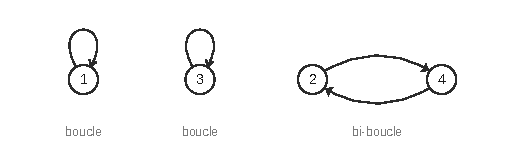
\includegraphics{figures/q26-graphe-permutation.pdf}
\caption*{Figure 3 --- Graphe G(σ) de la permutation de la figure 4 : boucles en 1
et 3, bi-boucle entre 2 et 4}
\end{figure}

\hypertarget{question-27}{%
\subsection{Question 27}\label{question-27}}

La figure 5 montre le cycle \(1\to2\to4\to3\to1\) et la boucle \(5\to5\). Donc :

\begin{longtable}[]{@{}llllll@{}}
\toprule\noalign{}
\(i\) & 1 & 2 & 3 & 4 & 5 \\
\midrule\noalign{}
\endhead
\bottomrule\noalign{}
\endlastfoot
\(\sigma(i)\) & 2 & 4 & 1 & 3 & 5 \\
\end{longtable}

\equationajustee{\boxed{M(\sigma)=\begin{pmatrix}0&1&0&0&0\\0&0&0&1&0\\1&0&0&0&0\\0&0&1&0&0\\0&0&0&0&1\end{pmatrix}.}}

\hypertarget{ii-propriuxe9tuxe9s}{%
\subsection{II --- Propriétés}\label{ii-propriuxe9tuxe9s}}

\hypertarget{question-28}{%
\subsection{Question 28}\label{question-28}}

Pour \(\tau\in\mathcal S_n\), \(M(\tau)_{i,j}=\delta_{j,\tau(i)}\) (symbole de Kronecker). Pour \((i,j)\in[\![1,n]\!]^2\) :
\equationajustee{\begin{aligned}
\big(M(\sigma)M(\sigma^{-1})\big)_{i,j}&=\sum_{k=1}^{n}\delta_{k,\sigma(i)}\,\delta_{j,\sigma^{-1}(k)}\\
&=\delta_{j,\sigma^{-1}(\sigma(i))}\\
&=\delta_{j,i},
\end{aligned}}
seul le terme \(k=\sigma(i)\) pouvant être non nul. Donc \(M(\sigma)M(\sigma^{-1})=I_n\). Une matrice carrée qui admet un inverse à droite est inversible, d'inverse celui-ci :
\equationajustee{\boxed{M(\sigma)^{-1}=M(\sigma^{-1}).}}

\hypertarget{question-29}{%
\subsection{Question 29}\label{question-29}}

Le graphe \(G(\sigma^{-1})\) a un arc \(i\to j\) si et seulement si \(\sigma^{-1}(i)=j\). Cela équivaut à \(\sigma(j)=i\), c'est-à-dire à l'existence de l'arc \(j\to i\) dans \(G(\sigma)\).

\textbf{\(G(\sigma^{-1})\) s'obtient en renversant tous les arcs de \(G(\sigma)\).}

De même, pour \((i,j)\in[\![1,n]\!]^2\) :
\equationajustee{\begin{aligned}
M(\sigma^{-1})_{i,j}=1&\iff\sigma^{-1}(i)=j\\
&\iff\sigma(j)=i\\
&\iff M(\sigma)_{j,i}=1.
\end{aligned}}
Les coefficients valant \(0\) ou \(1\), \textbf{\(M(\sigma^{-1})\) est la transposée de \(M(\sigma)\).} Avec Q28 :
\equationajustee{\boxed{M(\sigma)^{-1}=M(\sigma^{-1})=M(\sigma)^\top.}}

\hypertarget{question-30}{%
\subsection{Question 30}\label{question-30}}

\(\sigma^2=\sigma\circ\sigma\in\mathcal S_n\) et, pour \((i,j)\in[\![1,n]\!]^2\),
\equationajustee{\begin{aligned}
\big(M(\sigma)^2\big)_{i,j}&=\sum_{k=1}^{n}\delta_{k,\sigma(i)}\,\delta_{j,\sigma(k)}\\
&=\delta_{j,\sigma(\sigma(i))}\\
&=M(\sigma^2)_{i,j}.
\end{aligned}}
Donc \(\boxed{M(\sigma^2)=M(\sigma)^2.}\)

\hypertarget{iii-matrices-de-permutation-diagonalisables}{%
\subsection{III --- Matrices de permutation diagonalisables}\label{iii-matrices-de-permutation-diagonalisables}}

\hypertarget{question-31}{%
\subsection{Question 31}\label{question-31}}

« La matrice introduite en Q25 » est une coquille : il s'agit de la matrice \(N\) de la figure 4 (Q26), seule matrice \(4\times4\) compatible avec le polynôme annoncé.
\equationajustee{\begin{aligned}
\chi_N&=\det\begin{pmatrix}X-1&0&0&0\\0&X&0&-1\\0&0&X-1&0\\0&-1&0&X\end{pmatrix}\\
&=(X-1)^2\det\begin{pmatrix}X&-1\\-1&X\end{pmatrix}\\
&=(X-1)^2(X^2-1),
\end{aligned}}
en développant selon la première colonne puis selon la ligne de \(X-1\). Donc \(\boxed{\chi_N=(X-1)^3(X+1)}\).

\(N-I_4\) a deux lignes nulles et deux lignes opposées, \((0,-1,0,1)\) et \((0,1,0,-1)\). Donc \(\operatorname{rg}(N-I_4)=1\) et \(\dim\ker(N-I_4)=3\), égal à la multiplicité de \(1\).

Pour \(-1\), valeur propre simple, \(\dim\ker(N+I_4)=1\). La somme des dimensions vaut \(4\) : \textbf{\(N\) est diagonalisable.}

C'est cohérent avec le théorème : d'après Q26, \(G(\sigma)\) ne contient que deux boucles et une bi-boucle.

\hypertarget{question-32}{%
\subsection{Question 32}\label{question-32}}

\(M=M(\sigma)\) est supposée diagonalisable dans \(\mathcal M_n(\mathbb R)\) : ses valeurs propres sont réelles. Soit \(\lambda\) l'une d'elles et \(X\in\mathcal M_{n,1}(\mathbb R)\) non nul avec \(MX=\lambda X\). Par Q29, \(M^\top M=I_n\). Alors
\equationajustee{\begin{aligned}
\|X\|^2&=X^\top M^\top MX\\
&=(MX)^\top(MX)\\
&=\lambda^2\|X\|^2,
\end{aligned}}
et \(\|X\|^2>0\), donc \(\boxed{\lambda^2=1.}\)

\hypertarget{question-33}{%
\subsection{Question 33}\label{question-33}}

Il existe \(P\in GL_n(\mathbb R)\) et \(\Delta=\operatorname{diag}(\lambda_1,\dots,\lambda_n)\) telles que \(M(\sigma)=P\Delta P^{-1}\). Les \(\lambda_i\) sont les valeurs propres de \(M(\sigma)\) ; par Q32, \(\lambda_i\in\{-1,1\}\).

Soit \(q\in[\![0,n]\!]\) le nombre d'indices \(i\) tels que \(\lambda_i=1\). En réordonnant les colonnes de \(P\) (les vecteurs propres), on place ces valeurs en tête. Ainsi \textbf{\(M(\sigma)\) est semblable à \(\Delta_q\)}, où
\equationajustee{\Delta_q=\operatorname{diag}(\underbrace{1,\dots,1}_{q},\underbrace{-1,\dots,-1}_{n-q}).}

\hypertarget{question-34}{%
\subsection{Question 34}\label{question-34}}

\(\Delta_q^2=I_n\), donc \(M(\sigma)^2=P\Delta_q^2P^{-1}=I_n\). Par Q30 :
\equationajustee{\begin{aligned}
M(\sigma^2)&=M(\sigma)^2\\
&=I_n\\
&=M(\mathrm{id}).
\end{aligned}}
Comme \(M\) est injective, \(\boxed{\sigma^2=\mathrm{id}.}\)

Les arcs de \(G(\sigma)\) sont les \(i\to\sigma(i)\). Soit \(i\in[\![1,n]\!]\) et \(j=\sigma(i)\).

\begin{itemize}
\tightlist
\item
  Si \(j=i\), l'arc est une boucle.
\item
  Sinon \(\sigma(j)=\sigma^2(i)=i\). L'arc \(j\to i\) existe donc, et \(i\to j\to i\) est une bi-boucle.
\end{itemize}

\textbf{\(G(\sigma)\) ne contient que des boucles ou des bi-boucles.}

\hypertarget{question-35}{%
\subsection{Question 35}\label{question-35}}

Réciproquement, supposons que \(G(\sigma)\) ne contienne que des boucles et des bi-boucles. Soit \(i\in[\![1,n]\!]\) et \(j=\sigma(i)\).

\begin{itemize}
\tightlist
\item
  Si \(j=i\), alors \(\sigma^2(i)=i\).
\item
  Sinon, l'arc \(i\to j\) est dans une bi-boucle : \(\sigma(j)=i\), donc \(\sigma^2(i)=i\).
\end{itemize}

Ainsi \(\sigma^2=\mathrm{id}\). Notons \(M=M(\sigma)\) : par Q30, \(M^2=I_n\).

Soit \(x\in\mathcal M_{n,1}(\mathbb R)\). Posons
\equationajustee{\begin{aligned}
x_+&=\frac{x+Mx}2,\\
x_-&=\frac{x-Mx}2.
\end{aligned}}
Alors \(x=x_++x_-\). Comme \(M^2x=x\), on a \(Mx_+=x_+\) et \(Mx_-=-x_-\).

Notons \(E_{\pm1}=\ker(M\mp I_n)\). On a donc \(\mathcal M_{n,1}(\mathbb R)=E_1+E_{-1}\). La somme est directe, car \(Mx=x=-x\) impose \(x=0\).

Si \(E_1\) et \(E_{-1}\) sont non nuls, ce sont les deux sous-espaces propres de \(M\), de somme égale à l'espace : \(M\) est diagonalisable. Si l'un est nul, \(M=\pm I_n\) est diagonale.

Autre preuve, explicite. Comme \(\sigma=\sigma^{-1}\), on a \(Me_j=e_{\sigma(j)}\) pour tout \(j\).

\begin{itemize}
\tightlist
\item
  Pour chaque boucle \(i\), \(Me_i=e_i\).
\item
  Pour chaque bi-boucle \(\{i,j\}\), \(M(e_i+e_j)=e_i+e_j\) et \(M(e_i-e_j)=-(e_i-e_j)\).
\end{itemize}

Ces \(n\) vecteurs forment une base de vecteurs propres.

\textbf{\(M(\sigma)\) est diagonalisable}, ce qui achève la preuve du théorème : \(M(\sigma)\) est diagonalisable si et seulement si \(G(\sigma)\) ne contient que des boucles ou des bi-boucles.

\hypertarget{partie-d-graphes-de-permutations-sans-boucle}{%
\section{Partie D --- Graphes de permutations sans boucle}\label{partie-d-graphes-de-permutations-sans-boucle}}

\hypertarget{i-introduction}{%
\subsection{I --- Introduction}\label{i-introduction}}

\hypertarget{question-36}{%
\subsection{Question 36}\label{question-36}}

\(G\) est une bijection de \(\mathcal S_n\) sur \(G(\mathcal S_n)\), donc \(\boxed{|G(\mathcal S_n)|=|\mathcal S_n|=n!}\).

Une boucle de \(G(\sigma)\) est un point fixe de \(\sigma\) : \(X_n\) compte les points fixes.

Valeur exclue. Supposons que \(\sigma\) fixe exactement \(n-1\) éléments, et notons \(i_0\) l'élément restant. Son image ne peut être aucun des \(n-1\) autres, déjà atteints, car \(\sigma\) est injective. Donc \(\sigma(i_0)=i_0\) : contradiction.

Valeurs atteintes. Soit \(j\in[\![0,n]\!]\) avec \(j\neq n-1\), et \(m=n-j\). On fixe \(j\) éléments et l'on permute circulairement les \(m\) autres :
\equationajustee{c_1\to c_2\to\dots\to c_m\to c_1.}
Il n'y a pas de point fixe parmi eux si \(m\ge2\), et rien à faire si \(m=0\). Donc
\equationajustee{\boxed{X_n(\Omega)=[\![0,n]\!]\setminus\{n-1\}}}
(pour \(n=1\), cet ensemble est \(\{1\}\)).

\hypertarget{question-37}{%
\subsection{Question 37}\label{question-37}}

\textbf{Convention.} Avec \(b_0=0\), la formule serait fausse pour \(j=n\). En effet, l'identité est la seule permutation à \(n\) points fixes, donc \(P(X_n=n)=\frac1{n!}\). Or le membre de droite vaudrait \(\frac{b_0}{n!}=0\).

On adopte \(\boxed{b_0=1}\) (la permutation de l'ensemble vide n'a pas de point fixe) ; c'est la seule valeur qui rend vraies les formules de Q37 et Q38.

L'univers \(G(\mathcal S_n)\) est muni de la probabilité uniforme. Via \(G\), cela revient à tirer \(\sigma\) uniformément dans \(\mathcal S_n\). Soit \(j\in[\![0,n]\!]\). Une permutation à exactement \(j\) points fixes est déterminée par :

\begin{itemize}
\tightlist
\item
  l'ensemble \(F\) de ses points fixes, de cardinal \(j\) : \(\binom nj\) choix ;
\item
  sa restriction au complémentaire de \(F\), stable par \(\sigma\) et de cardinal \(n-j\). C'est une permutation sans point fixe : \(b_{n-j}\) choix, ce nombre ne dépendant que du cardinal.
\end{itemize}

Réciproquement, tout tel couple définit une permutation à exactement \(j\) points fixes. Donc
\equationajustee{\boxed{\forall j\in[\![0,n]\!],\ \ P(X_n=j)=\frac{\binom nj\,b_{n-j}}{n!}.}}

\hypertarget{question-38}{%
\subsection{Question 38}\label{question-38}}

Les événements \((X_n=j)\), \(j\in[\![0,n]\!]\), forment un système complet (celui d'indice \(n-1\) étant impossible). Donc
\equationajustee{1=\sum_{j=0}^{n}\frac{\binom nj\,b_{n-j}}{n!}.}
En multipliant par \(n!\), avec \(\binom nj=\binom n{n-j}\) puis \(k=n-j\) :
\equationajustee{\begin{aligned}
n!&=\sum_{j=0}^{n}\binom n{n-j}b_{n-j}\\
&=\sum_{k=0}^{n}\binom nk b_k.
\end{aligned}}
Les \(b_k\) ne dépendent pas de \(n\). En effet, \(b_k\) est le nombre de permutations sans point fixe d'un ensemble à \(k\) éléments.

Pour \(p\in[\![1,n]\!]\), le même raisonnement dans \(\mathcal S_p\) donne la relation au rang \(p\). Pour \(p=0\), elle s'écrit \(0!=b_0\), vraie avec \(b_0=1\). Donc
\equationajustee{\boxed{\forall p\in[\![0,n]\!],\ \ p!=\sum_{k=0}^{p}\binom pk b_k.}}

\hypertarget{question-39}{%
\subsection{Question 39}\label{question-39}}

Le terme \(k=p\) ayant pour coefficient \(\binom pp=1\), la relation au rang \(p\ge1\) s'écrit
\equationajustee{b_p=p!-\sum_{k=0}^{p-1}\binom pk b_k.}
Partant de \(b_0=1\), elle détermine de proche en proche \(b_1,\dots,b_n\) (système triangulaire à diagonale de \(1\)). On obtient
\equationajustee{\begin{aligned}
b_1&=1-1\\
&=0,\\[4pt]
b_2&=2-1-2\cdot0\\
&=1,\\[4pt]
b_3&=6-1-3\cdot0-3\cdot1\\
&=2.
\end{aligned}}
Ainsi \(\boxed{b_1=0,\ b_2=1,\ b_3=2.}\) (Contrôle : sur \([\![1,3]\!]\), seuls les deux \(3\)-cycles sont sans point fixe.)

\hypertarget{ii-calcul-dune-probabilituxe9-par-deux-muxe9thodes}{%
\subsection{II --- Calcul d'une probabilité par deux méthodes}\label{ii-calcul-dune-probabilituxe9-par-deux-muxe9thodes}}

\hypertarget{question-40}{%
\subsection{Question 40}\label{question-40}}

L'étude de la série entière de somme \(s\) a fourni (Q25), pour tout \(p\) :
\equationajustee{p!=\sum_{k=0}^{p}\binom pk a_k.}
Q38 donne la même relation pour les \(b_k\), pour \(p\in[\![0,n]\!]\).

Montrons par récurrence forte que \(a_p=b_p\) pour \(p\in[\![0,n]\!]\).

\begin{itemize}
\tightlist
\item
  En \(p=0\) : \(a_0=b_0=1\).
\item
  Si \(a_k=b_k\) pour \(k<p\), la différence des deux relations au rang \(p\) donne \(0=\binom pp(a_p-b_p)=a_p-b_p\).
\end{itemize}

Donc \(b_n=a_n=n!S_n\) (Q21). Comme \(B_n=(X_n=0)\) a pour cardinal \(b_n\) dans un univers équiprobable de cardinal \(n!\) :
\equationajustee{\boxed{\begin{aligned}
P(B_n)&=\frac{b_n}{n!}\\
&=S_n\\
&=\sum_{k=0}^{n}\frac{(-1)^k}{k!}.
\end{aligned}}}

\hypertarget{question-41}{%
\subsection{Question 41}\label{question-41}}

\(L\) est inversible et \((L^{-1})_{i,j}=(-1)^{i-j}\binom ij\) (Q7). Pour \(i\in[\![0,n]\!]\) :
\equationajustee{\begin{aligned}
(L^{-1}F)_i&=\sum_{j=0}^{i}(-1)^{i-j}\frac{i!}{j!\,(i-j)!}\,j!\\
&=i!\sum_{j=0}^{i}\frac{(-1)^{i-j}}{(i-j)!}\\
&=i!\sum_{m=0}^{i}\frac{(-1)^m}{m!}\\
&=i!\,S_i,
\end{aligned}}
\equationajustee{\boxed{L^{-1}F=\begin{pmatrix}0!\,S_0\\1!\,S_1\\\vdots\\n!\,S_n\end{pmatrix}.}}
Posons \(B=(b_0,\dots,b_n)^\top\). Pour \(i\in[\![0,n]\!]\), Q38 donne
\equationajustee{\begin{aligned}
(LB)_i&=\sum_{j=0}^{i}\binom ij b_j\\
&=i!\\
&=F_i.
\end{aligned}}
Donc \(LB=F\), puis \(B=L^{-1}F\) : \(b_i=i!\,S_i\) pour tout \(i\). En particulier
\equationajustee{\boxed{\begin{aligned}
P(B_n)&=\frac{b_n}{n!}\\
&=\sum_{k=0}^{n}\frac{(-1)^k}{k!},
\end{aligned}}}
retrouvé sans utiliser la partie B.

\end{document}
